% End-to-end attack F1 across VLM variants (HF-GradInv, no defense).
% Mean over 3 seeds (42, 123, 256), error bars = std.
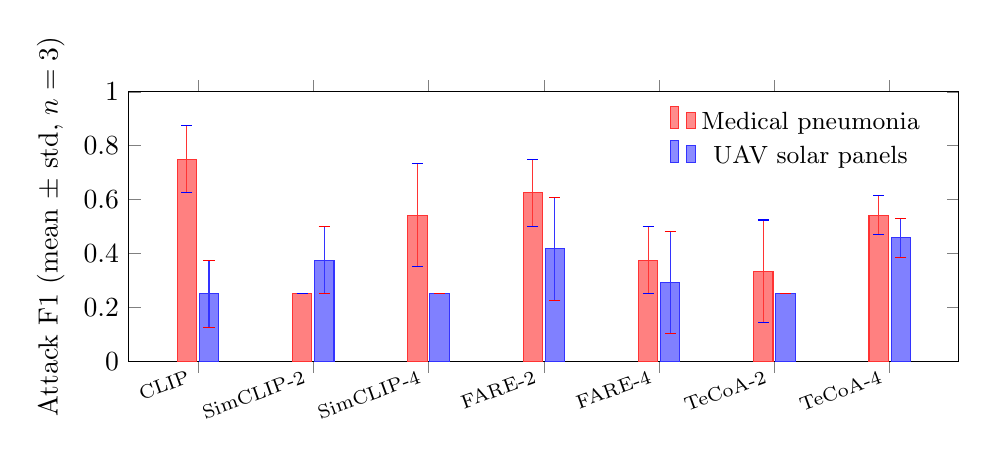
\begin{tikzpicture}
\begin{axis}[
    width=\columnwidth,
    height=5cm,
    ybar=1pt,
    bar width=7pt,
    enlarge x limits=0.10,
    ylabel={Attack F1 (mean $\pm$ std, $n=3$)},
    symbolic x coords={CLIP, SimCLIP-2, SimCLIP-4, FARE-2, FARE-4, TeCoA-2, TeCoA-4},
    xtick=data,
    xticklabel style={font=\scriptsize, rotate=20, anchor=east},
    ymin=0, ymax=1.0,
    legend pos=north east,
    legend style={font=\small, draw=none, fill=white, fill opacity=0.9, text opacity=1},
    error bars/y dir=both,
    error bars/y explicit,
]
\addplot+[fill=red!50, draw=red!80] coordinates {
    (CLIP, 0.750) +- (0,0.125)
    (SimCLIP-2, 0.250) +- (0,0.000)
    (SimCLIP-4, 0.542) +- (0,0.191)
    (FARE-2, 0.625) +- (0,0.125)
    (FARE-4, 0.375) +- (0,0.125)
    (TeCoA-2, 0.333) +- (0,0.191)
    (TeCoA-4, 0.542) +- (0,0.072)
};
\addlegendentry{Medical pneumonia}
\addplot+[fill=blue!50, draw=blue!80] coordinates {
    (CLIP, 0.250) +- (0,0.125)
    (SimCLIP-2, 0.375) +- (0,0.125)
    (SimCLIP-4, 0.250) +- (0,0.000)
    (FARE-2, 0.417) +- (0,0.191)
    (FARE-4, 0.292) +- (0,0.191)
    (TeCoA-2, 0.250) +- (0,0.000)
    (TeCoA-4, 0.458) +- (0,0.072)
};
\addlegendentry{UAV solar panels}
\end{axis}
\end{tikzpicture}
